\documentclass{article}

\usepackage[margin=1in]{geometry}
\usepackage{amsmath,amsthm,amssymb}
\usepackage{bbm, enumerate, tikz}
\usepackage{multicol}

\newenvironment{problem}[2][Problem]{\begin{trivlist}
\item[\hskip \labelsep {\bfseries #1}\hskip \labelsep {\bfseries #2.}]}{\end{trivlist}}
\newenvironment{note}[1][Note.]{\begin{trivlist}
\item[\hskip \labelsep {\bfseries #1}]}{\end{trivlist}}

\begin{document}

\title{Spring 2014: Complex Analysis Graduate Exam}
\author{Peter Kagey}

\maketitle

% -----------------------------------------------------
% First problems
% -----------------------------------------------------
\begin{problem}{1}
  For $a > 0$, evaluate the integral \[
    \int_0^\infty \frac{\log x}{(a + x)^3}\, dx
  \] being careful to justify your methods.
\end{problem}

\begin{proof}
  First, call this integral $S$, and denote the integrand by $f(x)$.
  We will evaluate this integral using the usual trick: integrating
  $g(z) = f(z)\log(z)$ around a keyhole contour, with the branch cut of
  the logarithm along the positive real axis, so that the contour contains the
  pole at $z = -a$.

  \begin{multicols}{2}
  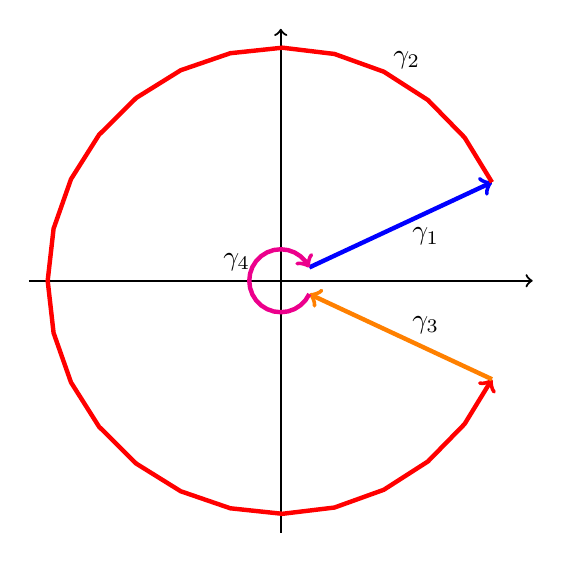
\begin{tikzpicture}[scale=0.8]
    % \draw[very thin,color=gray] (-0.9,-0.9) grid (5.9,5.9);
    \draw[thick, ->] (-4,0)--(4,0);
    \draw[thick, ->] (0,-4)--(0,4);
    \draw[ultra thick, ->, draw=blue, domain=0.5:3.7] plot ({\x*cos(25)}, {\x*sin(25)});
    \draw node at (2.3, 0.7) {$\gamma_{1}$};
    \draw[ultra thick, ->, draw=red, domain=25:335] plot ({3.7*cos(\x)}, {3.7*sin(\x)});
    \draw node at (2, 3.5) {$\gamma_{2}$};
    \draw[ultra thick, ->, draw=orange, domain=3.7:0.5] plot ({\x*cos(25)}, {-\x*sin(25)});
    \draw node at (2.3, -0.7) {$\gamma_{3}$};
    \draw[ultra thick, ->, draw=magenta, domain=335:25] plot ({0.5*cos(\x)}, {0.5*sin(\x)});
    \draw node at (-0.7, 0.3) {$\gamma_{4}$};
  \end{tikzpicture}\\
  \begin{align}
    \gamma_{1} &= \{te^{i\rho}\ |\ t \in [\varepsilon, R] \} \\
    \gamma_{2} &= \{R e^{it}\ |\ t \in [\rho,2\pi-\rho] \} \\
    \gamma_{3} &= \{-te^{(2\pi -\rho)i}\ |\ t \in [-R, -\varepsilon]\} \\
    \gamma_{4} &= \{\varepsilon e^{-it}\ |\ t \in [-2\pi + \rho, -\rho]\}.
  \end{align}
  \end{multicols}

  Then by the residue theorem, \[
    \int_{\gamma_1} g(z) dz + \int_{\gamma_2} g(z) dz + \int_{\gamma_3} g(z) dz + \int_{\gamma_4} g(z) dz
    = \operatorname{Res}_{-a}(g).
  \]
  As expected, the integrals along the arcs vanish in the limit.
  \\
  Firstly, the large arc is bounded by \begin{align*}
    \left|
      \int_{\gamma_2} g(z) dz
    \right|
    &\leq \int_0^{2\pi} \left|
      \frac{\log^2(Re^{i\theta})}{(a + Re^{i\theta})^3}Rie^{i\theta}
    \right| d\theta \\s
    &\leq \int_0^{2\pi} \left|
      \frac{\log^2(Re^{i\theta})}{R^3e^{3i\theta}}R
    \right| d\theta \\
    &\leq \int_0^{2\pi} \left|
      \frac{\log^2 R + 2i\theta\log R - \theta}{R^2}
    \right| d\theta,
  \end{align*} which vanishes as $R \rightarrow \infty$ by the ML inequality.
  Next, the small arc is bounded by \begin{align*}
    \left|
      \int_{\gamma_4} g(z) dz
    \right|
    &\leq \int_0^{2\pi} \left|
      \frac{\log^2(\rho e^{i\theta})}{(a + \rho e^{i\theta})^3}\rho ie^{i\theta}
    \right| d\theta \\
    &\leq \int_0^{2\pi} \left|
      \frac{\log^2(\rho e^{i\theta})}{(a/2)^3}\rho
    \right| d\theta \\
    &\leq \frac{8}{a^3}\int_0^{2\pi} \left|
      \rho(\log^2\rho + 2i\theta\log\rho - \theta)
    \right| d\theta,
  \end{align*} which vanishes as $\rho \rightarrow 0$ with the ML inequality
  together with two applications of L'H\^opital's rule \[
    \lim_{\rho \rightarrow 0} \rho\log^2 \rho
    = \lim_{\rho \rightarrow 0} \frac{\log^2 \rho}{\rho^{-1}}
    = \lim_{\rho \rightarrow 0} \frac{2\rho^{-1}\log \rho}{-\rho^{-2}}
    = \lim_{\rho \rightarrow 0} \frac{2\log \rho}{-\rho^{-1}}
    = \lim_{\rho \rightarrow 0} \frac{2\rho^{-1}}{\rho^{-2}}
    = \lim_{\rho \rightarrow 0} 2\rho
    = 0.
  \]
  Now the integral has been reduced to \[
    \int_{\gamma_1} g(z) dz + \int_{\gamma_3} g(z) dz = \operatorname{Res}_{-a}(g).
  \]
  Evaluating the remaining integrals yields \begin{align*}
    \int_{\gamma_1} g(z) dz + \int_{\gamma_3} g(z)
    &=
    \lim_{\rho \rightarrow 0}
    \int_\varepsilon^R \frac{\log^2(te^{i\rho})}{(a + te^{i\rho})^3}e^{i\rho}dt +
    \int_R^\varepsilon \frac{\log^2(te^{i(2\pi-\rho)})}{(a + te^{i(2\pi-\rho)})^3}e^{i(2\pi-\rho)}dt \\
    &=
    \int_\varepsilon^R \frac{\log^2(t)}{(a + t)^3}dt +
    \int_R^\varepsilon \frac{(\log(t) + 2\pi i)^2}{(a + t)^3}dt \\
    &=
    \int_\varepsilon^R \frac{4\pi^2 - 4\pi i\log(t)}{(a + t)^3}dt \\
    &=
    \int_\varepsilon^R \frac{4\pi^2}{(a + t)^3}dt - 4\pi i\int_\varepsilon^R \frac{\log(t)}{(a + t)^3}dt.
  \end{align*}
  Using ordinary techniques of integration, we can evaluate the integral \[
    \int_0^\infty \frac{4\pi^2}{(a + t)^3}dt = \left[\frac{4\pi^2}{-2(a - t)^2}\right]_0^\infty = \frac{2\pi^2}{a^2}.
  \]
  Computing the residue of $g$ at $z = -a$ just requires computing the Taylor
  series of $\log^2z$ centered at $z = -a$ to a second order term, which requires
  computing the second derivative of $\log^2 z$. \begin{align*}
    \frac{d}{dz}[\log^2 z] &= 2\log(z)z^{-1} \\
    \frac{d^2}{dz^2}[\log^2 z] &= 2(-\log(z)z^{-2} + z^{-2})
  \end{align*}
  Thus \[
    \frac{\log^2 z}{(z + a)^3} = \frac{1}{(z + a)^3} = \left[
      \log^2(-a)
      + \frac{2\log(-a)}{-a}(z + a)
      + \frac{2(1 - \log(-a))}{2a^{2}}(z + a)^2
      + \hdots
    \right].
  \]
  So the residue at $z = -a$ is \[
    \operatorname{Res}_{-a}(g)
    = \frac{1 - \log(-a)}{a^{2}}
    = \frac{1 - \log(a) - \log(-1)}{a^{2}}
    = \frac{1 - \log(a) - \pi i}{a^{2}}.
  \]
  Now we have all of the ingredients to compute the integral: \begin{align*}
  \frac{2\pi^2}{a^2} - 4\pi i\int_0^\infty \frac{\log(t)}{(a + t)^3}dt &= 2\pi i \left(\frac{1 - \log(a) - \pi i}{a^{2}}\right) \\
  \int_0^\infty \frac{\log(t)}{(a + t)^3}dt &= \frac{1}{4\pi i}\left(\frac{2\pi^2}{a^2} - \frac{2\pi i(1 - \log(a) - \pi i)}{a^{2}}\right)
  = \frac{\log(a) - 1}{2a^2}.
  \end{align*}
\end{proof}

% -----------------------------------------------------
% Second problem
% -----------------------------------------------------
\pagebreak

\begin{problem}{2}
  Find a conformal mapping of the region
  $\{ z : |z| > 1 \} \setminus (1, \infty)$
  onto the open unit disk $\{ z : |z| < 1\}$.
\end{problem}

\begin{proof}
  $ $ \\
  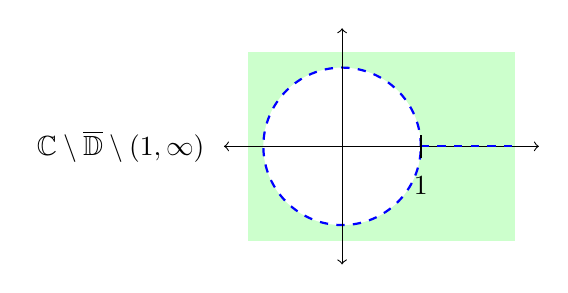
\begin{tikzpicture}
    \node[anchor=west] at (-4, 0) {$\mathbb{C} \setminus \overline{\mathbb{D}} \setminus (1, \infty)$};
    \fill[green, opacity=0.2] (-1.2,-1.2) rectangle (2.2,1.2);
    \draw[blue, fill=white, thick, dashed] (0,0) circle (1);
    \draw[<->] (-1.5,0)--(2.5,0);
    \draw[<->] (0,-1.5)--(0,1.5);
    \draw[blue, thick, dashed] (1,0)--(2.2,0);
    \draw[thick] (1,-0.15)--(1,0.15);
    \node at (1,-0.5) {1};
  \end{tikzpicture}
  \hspace{0.7cm}
  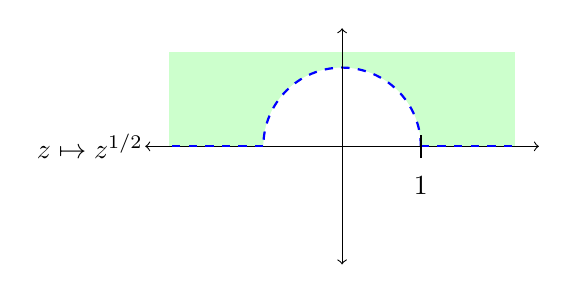
\begin{tikzpicture}
    \node[anchor=west] at (-4, 0) {$z \mapsto z^{1/2}$};
    \fill[green, opacity=0.2] (-2.2,0) rectangle (2.2,1.2);
    \draw[blue, fill=white, thick, dashed] (1,0) arc (0:180:1);
    \draw[<->] (-2.5,0)--(2.5,0);
    \draw[<->] (0,-1.5)--(0,1.5);
    \draw[blue, thick, dashed] (1,0)--(2.2,0);
    \draw[blue, thick, dashed] (-1,0)--(-2.2,0);
    \draw[thick] (1,-0.15)--(1,0.15);
    \node at (1,-0.5) {1};
  \end{tikzpicture}
  \\
  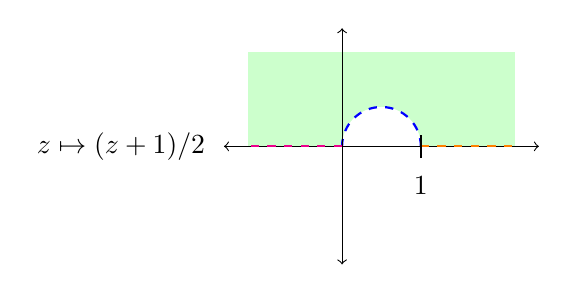
\begin{tikzpicture}
    \node[anchor=west] at (-4, 0) {$z \mapsto (z + 1)/2$};
    \fill[green, opacity=0.2] (-1.2,0) rectangle (2.2,1.2);
    \draw[blue, fill=white, thick, dashed] (1,0) arc (0:180:0.5);
    \draw[<->] (-1.5,0)--(2.5,0);
    \draw[<->] (0,-1.5)--(0,1.5);
    \draw[orange, thick, dashed] (1,0)--(2.2,0);
    \draw[magenta, thick, dashed] (0,0)--(-1.2,0);
    \draw[thick] (1,-0.15)--(1,0.15);
    \node at (1,-0.5) {1};
  \end{tikzpicture}
  \hspace{0.7cm}
  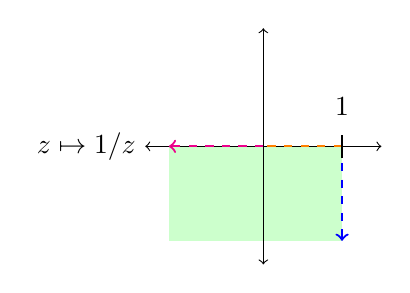
\begin{tikzpicture}
    \node[anchor=west] at (-3, 0) {$z \mapsto 1/z$};
    \fill[green, opacity=0.2] (1,0) rectangle (-1.2,-1.2);
    \draw[<->] (-1.5,0)--(1.5,0);
    \draw[<->] (0,-1.5)--(0,1.5);
    \draw[thick, dashed, orange] (1,0)--(0,0);
    \draw[thick, dashed, magenta, ->] (0,0)--(-1.2,0);
    \draw[thick, dashed, blue, ->] (1,0)--(1,-1.2);
    \draw[thick] (1,-0.15)--(1,0.15);
    \node at (1,0.5) {1};
  \end{tikzpicture}
  \\
  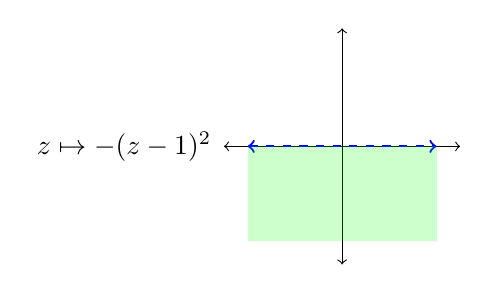
\begin{tikzpicture}
    \node[anchor=west] at (-4, 0) {$z \mapsto -(z - 1)^2$};
    \draw[<->] (-1.5,0)--(1.5,0);
    \draw[<->] (0,-1.5)--(0,1.5);
    \draw[thick, dashed, blue, <->] (-1.2,0)--(1.2,0);
    \fill[green, opacity=0.2] (-1.2,0) rectangle (1.2,-1.2);
  \end{tikzpicture}
  \hspace{0.7cm}
  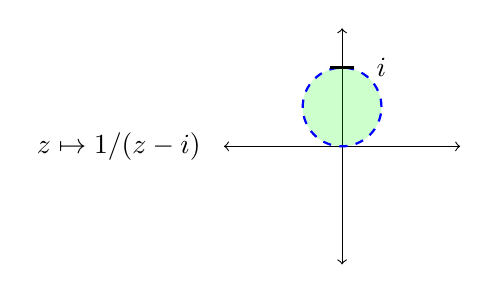
\begin{tikzpicture}
    \node[anchor=west] at (-4, 0) {$z \mapsto 1/(z - i)$};
    \draw[<->] (-1.5,0)--(1.5,0);
    \draw[<->] (0,-1.5)--(0,1.5);
    % \draw[]
    \draw[thick, dashed, blue, fill=green, fill opacity=0.2] (0,0.5) circle (0.5);
    % \fill[green, opacity=0.2] (-1.2,0) rectangle (1.2,-1.2);
    \draw[thick] (-0.15,1)--(0.15,1);
    \node at (0.5, 1) {$i$};
  \end{tikzpicture}
  \\
  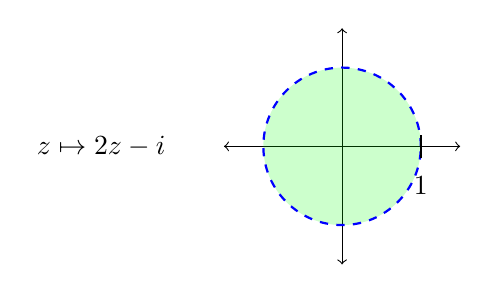
\begin{tikzpicture}
    \node[anchor=west] at (-4, 0) {$z \mapsto 2z - i$};
    \draw[<->] (-1.5,0)--(1.5,0);
    \draw[<->] (0,-1.5)--(0,1.5);
    \draw[blue, fill=green, fill opacity=0.2, thick, dashed] (0,0) circle (1);
    % \draw[blue, thick, dashed] (0,0)--(1,0);
    \draw[thick] (1,-0.15)--(1,0.15);
    \node at (1,-0.5) {1};
  \end{tikzpicture}
\end{proof}

% -----------------------------------------------------
% Third problem
% -----------------------------------------------------
\pagebreak

\begin{problem}{3}
  Suppose that $f_n$ are analytic functions on a connected open set
  $U \subset \mathbb{C}$ and that $f_n \rightarrow f$ uniformly on compact
  subsets of $U$. In each case indicate the main steps in the proofs of the
  following standard results. \begin{enumerate}[(i)]
    \item $f$ is analytic in $U$;
    \item $f'_n \rightarrow f'$ uniformly on compact subsets of $U$;
    \item if $f_n(z) \neq 0$ for all $n$ and all $z \in U$, then either
      $f(z) \neq 0$ for all $z \in U$ or else $f \equiv 0$.
  \end{enumerate}
\end{problem}

\begin{proof}
\end{proof}

% -----------------------------------------------------
% Fourth problem
% -----------------------------------------------------
\pagebreak

\begin{problem}{4} $ $\\
  \begin{enumerate}[(a)]
    \item Suppose that $f$ is analytic on the open unit disk $\{ z : |z| < 1 \}$
    and that there exists a constant $M$ such that $|f^k(0)| \leq k^4 M^k$ for
    all $k \geq 0$. Show that $f$ can be extended to be analytic on
    $\mathbb{C}$.
    \item Suppose that $f$ is analytic on the open unit disk and that there
    exists a constant $M > 1$ such that $|f(1/k)| \leq M^{-k}$ for all
    $k \geq 1$. Show that $f$ is identically zero.
  \end{enumerate}
\end{problem}

\begin{proof}
\end{proof}

\end{document}
